\section{\bench 基准}
\label{sec:bench}

\begin{figure*}[t]
\centering
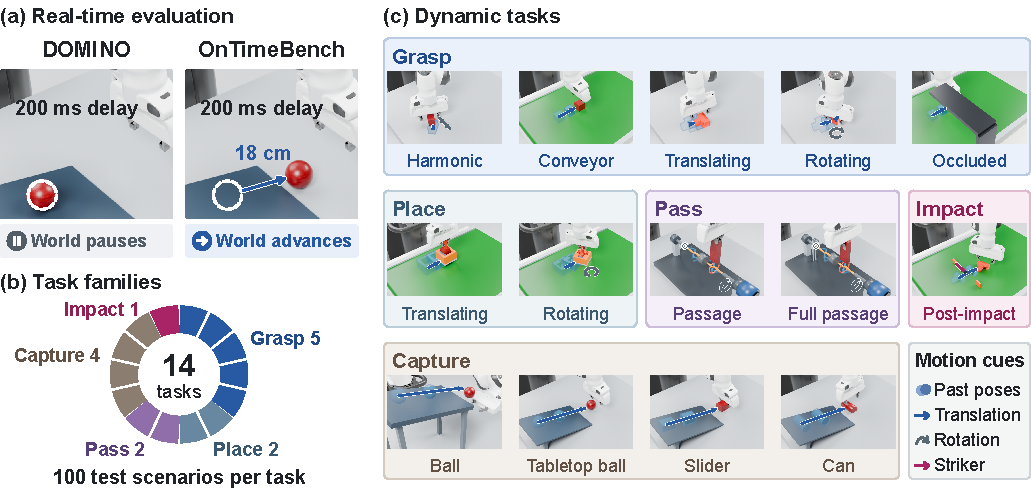
\includegraphics[width=\textwidth]{figures/Fig4/ontimebench.pdf}
\caption{\textbf{\bench 总览。}\bench 在各方法的原生延迟下评测策略，包含五个任务族共 14 个动态任务和 1{,}400 个留出测试场景。
(a) DOMINO~\cite{domino} 在推理期间暂停世界，\bench 则让世界持续运动。
(b) 任务族分布。(c) 任务展示。}
\label{fig:bench_overview}
\end{figure*}


\subsection{概览}
\label{sec:bench_overview}
动态基准必须让每个策略为其计算所花的时间付出代价。如果仿真要等策略返回动作之后才推进，如 DOMINO \cite{domino} 与 PhysMani-Bench \cite{physmani} 的默认评测器那样，慢的策略就被当作瞬时完成来评分：这样的评测衡量了策略预测了什么，却没有衡量预测能否及时到达，而后者正是真机上成败的关键。

为了评测策略能否及时作用于运动中的场景，我们提出 \bench，一个包含 14 个动态操作任务的基准，其中世界从不暂停。观测、场景运动与动作执行共用一个物理时钟，因此每个策略计算多久，场景就继续运动多久。图~\ref{fig:bench_overview}(a) 展示了这一差别：在 200\,ms 的推理期间，世界暂停时滚动的小球停在被观测到的位置；而在 \bench 中它已经滚出 18\,cm，瞄准观测位置的动作会落空。\bench 包含五个任务族（图~\ref{fig:bench_overview}(b)）：\emph{抓取}，抓取做简谐、传送带、平移、旋转或遮挡运动的目标；\emph{放置}，把所持物体放入平移或旋转的容器；\emph{穿越}，让棒沿旋转的导线穿过；\emph{捕获}，捕获滚动或滑动的物体；以及\emph{撞击}，在撞击后抓取零件。图~\ref{fig:bench_overview}(c) 展示了全部 14 个任务。这些任务共同改变决定成败的因素：目标的速度（0.03 至 1.14\,m/s）、目标的旋转、障碍物留出的间隙，以及传送带、斜坡、撞击器等驱动物传递的运动。

\subsection{构建}
\label{sec:bench_construction}
\bench 基于 MuJoCo 与 robosuite \cite{mujoco,robosuite} 构建，使用以 \cfgControlRate{} 控制的 Franka Panda 机械臂。每个场景在任务各自的范围内采样目标的初始状态与运动参数。使用仿真特权状态的任务专家为每个任务提供 \cfgDemos{} 条示范，共 11{,}200 条。所有结果都在全部方法共用的 1{,}400 个留出测试场景（每个任务 100 个）上报告；配置在另外的开发场景上选择。

\subsection{评测协议}
\label{sec:bench_protocol}
\paragraph{原生延迟。}
每次查询期间，物理按该方法自身的推理延迟推进；延迟从该方法在一块 \cfgGPU{} 上以 batch 1 实测的延迟分布中抽取。所有方法共用同一个执行器：它在推理完成后的第一个控制周期边界接收动作块，并从对应该边界的指令开始执行。

\paragraph{设置与指标。}
我们评测三种设置：\emph{原生}，各方法承担自身的延迟；\emph{+150\,ms}，为每个方法附加 150\,ms；以及\emph{暂停}，在推理期间暂停世界。我们报告任务等权的成功率（SR）与 p95 出动作时间，即从采集观测到其第一条指令可用的时间。完整协议见补充材料。
